\documentclass[border=10pt]{standalone}
\usepackage{tikz}
\usetikzlibrary{positioning}
\begin{document}
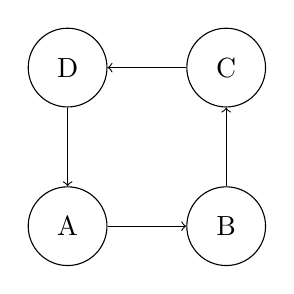
\begin{tikzpicture}[every node/.style={circle, draw, minimum size=1cm}]
  \node (a) {A};
  \node[right=of a] (b) {B};
  \node[above=of b] (c) {C};
  \node[left=of c] (d) {D};
  \draw[->] (a) -- (b);
  \draw[->] (b) -- (c);
  \draw[->] (c) -- (d);
  \draw[->] (d) -- (a);
\end{tikzpicture}
\end{document}
